\section{用户故事}

\subsection{任务发布方用户故事}

作为一个大规模数据的需求者,我希望能够通过该平台便捷地发布数据标注任务,并获取大量优质可靠的数据结果。我愿意为这些标注者支付报酬,但前提是他们提供的数据正确可靠。我希望能够快速、便捷地注册,不希望浪费太多时间完成审核认证。另外,我希望我在平台上付出的成本低于或等于我支付给其他数据标注人员(企业员工)的成本,不然这个平台就会失去它的价值。在发布任务时,我也希望平台能给我清晰地引导,并满足我任务所需的数据格式要求。

\subsection{任务接收方用户故事}

作为一名互联网用户,我希望能够利用空余时间便捷地完成一些任务,并为我付出的劳动获取相应的报酬。由于我许多的空余时间都是碎片化的,因此我希望单项任务耗费的时间不要太长。在交互方面,我希望任务的流程指示清晰、明确、易懂,不希望为了理解软件的使用方法而浪费太多时间。在视觉方面,我希望平台界面设计的观感舒适美观。最后,我希望我的报酬可以便捷、直接地提现,转换成我的个人财富。

\subsection{用户故事优先级}

\begin{figure}[h!]
    \centering
    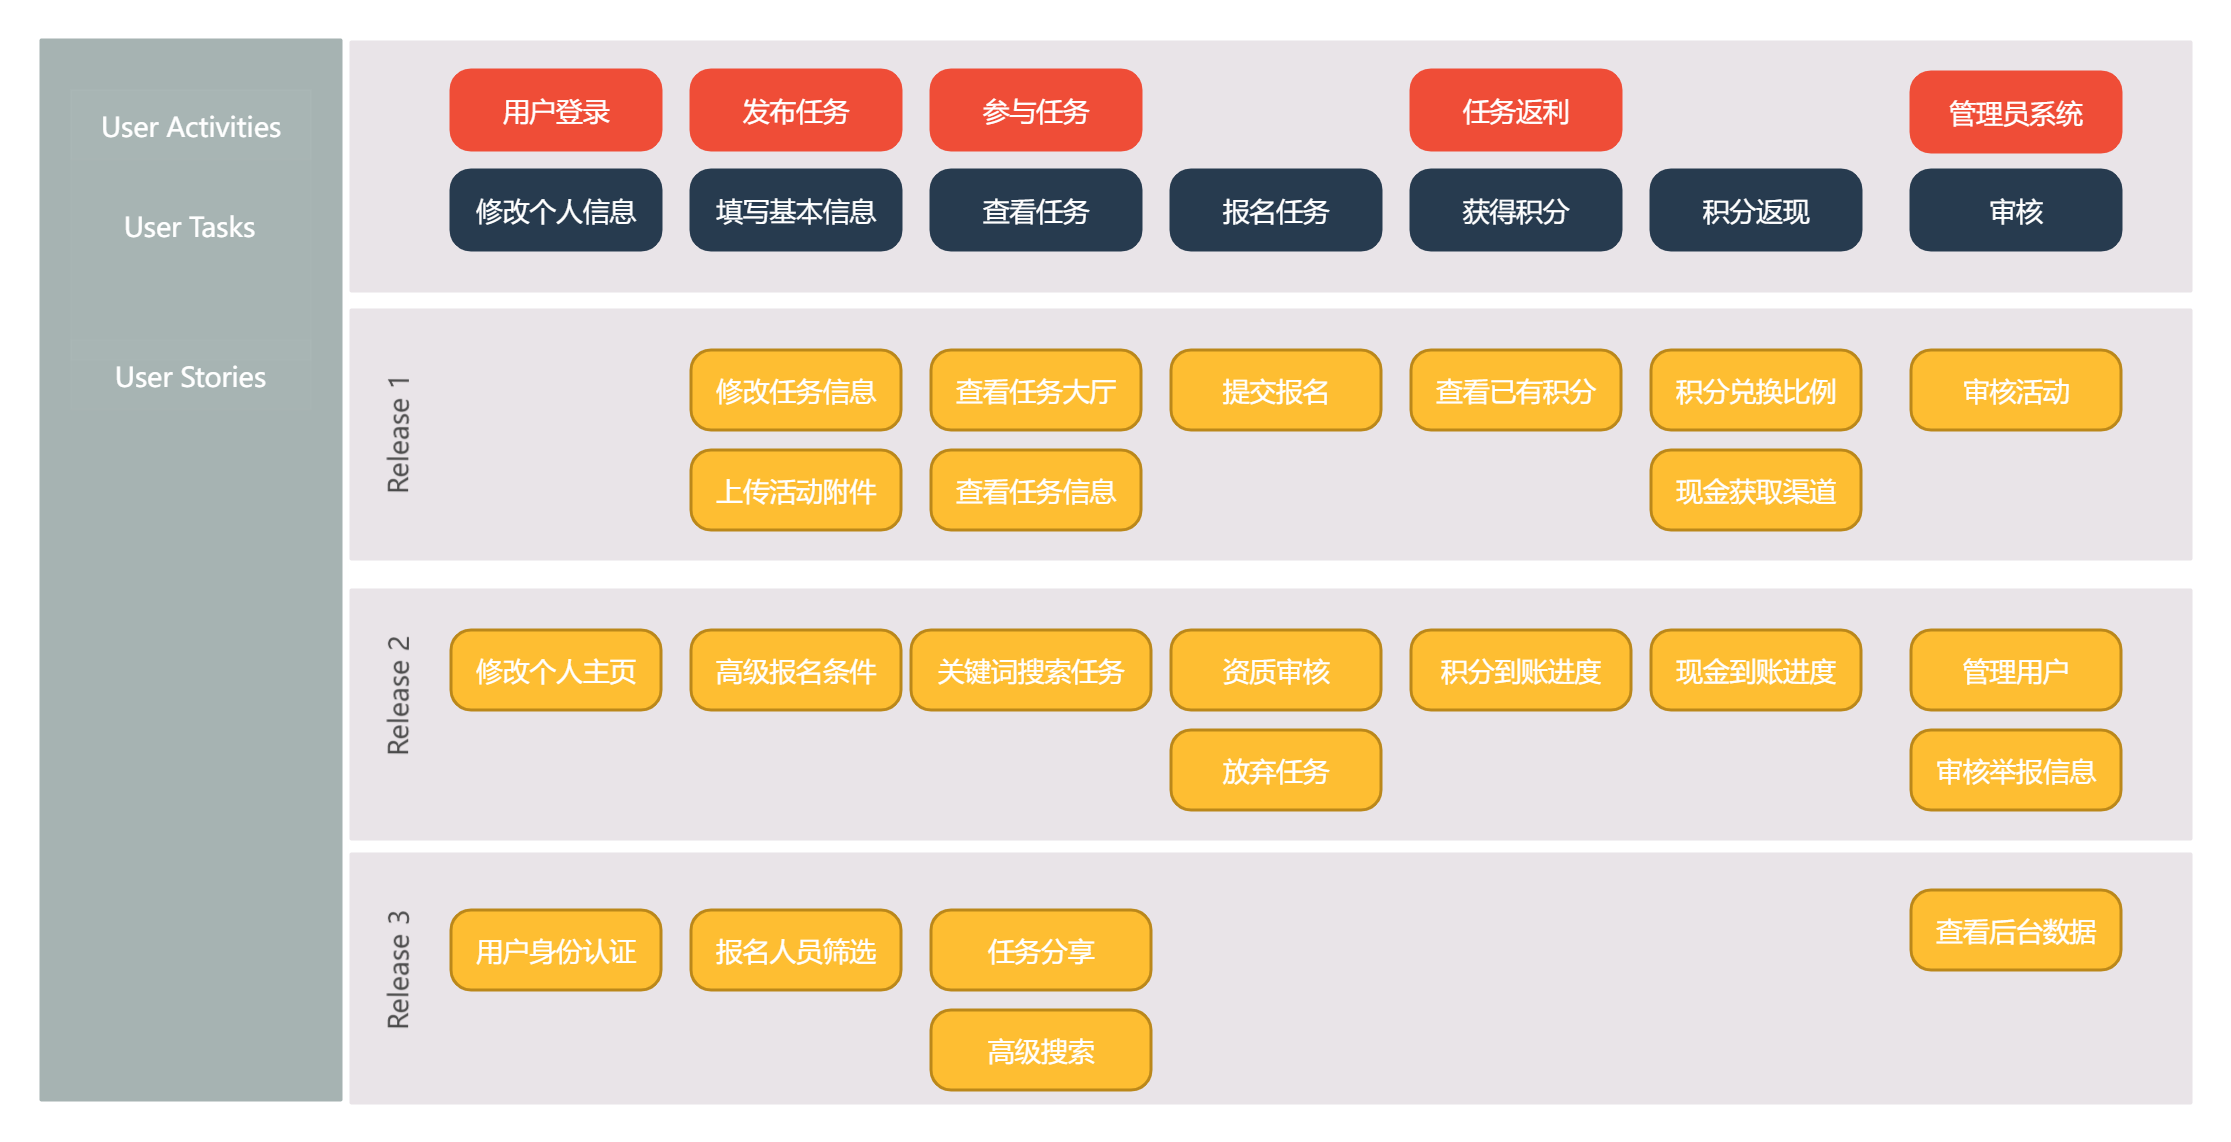
\includegraphics[width=\linewidth]{imgs/roadmap.png}
    \caption{用户故事优先级}
\end{figure}